\chapter{A NON-UNIFORM REFINEMENT APPROACH
FOR SOLVING ADJOINT PROBLEMS IN FUNCTIONAL
ERROR ESTIMATION AND MESH ADAPTATION}
\label{chap:refine}

%%% INTRODUCTION
\section{Introduction}

Adjoint-based error estimation
\cite{becker2001optimal, giles2003adjoint,
pierce2004adjoint, venditti2000adjoint,
venditti2002adjoint,
venditti2003adjoint,
prudhomme1999goal,
prudhomme2003practical,
fidkowski2011review,
connors2013method}
is a tool used in numerical simulation
to estimate the discretization error
in physically meaningful output quantities.
Combined with mesh adaptation, adjoint-based error
estimation also provides the ability to control the discretization
error. The process of adjoint-based error estimation
relies on the introduction of an auxiliary
\emph{adjoint problem}, which is constructed using
the solution to the original or \emph{primal problem}
of interest.

To obtain meaningful error estimates,
the solution to the adjoint problem must be
enriched in some manner. That is, it is
necessary to obtain a representation of the
adjoint solution in a richer space compared
to the space used for the primal problem.
Several strategies are commonly used
to obtain an enriched adjoint representation.
These approaches include
solving the adjoint problem in a globally higher
order polynomial space
\cite{fidkowski2011output},
solving the adjoint problem on a uniformly
refined mesh \cite{burstedde2009parallel},
solving the adjoint problem in the same space
as used for the primal problem
and solving local patch-wise problems least
squares problems \cite{nemec2007adjoint} or
performing patch-wise higher-order interpolation
\cite{becker2001optimal},
and enriching the adjoint solution via
variational multiscale methods
\cite{granzow2017output}.

Solving the adjoint problem in a globally higher
order polynomial space or on a uniformly refined mesh
is a computationally expensive proposition. On the
other hand, solving the adjoint problem in the same
space as used for the primal problem and enriching
it via some local recovery operation may not be guaranteed
to yield a more accurate adjoint solution. In this
chapter, we propose a simple compromise and solve the
adjoint problem on meshes obtained via non-uniform
refinement.

The remainder of this chapter is structured as follows.
First, we review adjoint-based error estimation for
functional quantities using two discretization levels,
a \emph{coarse} space and a \emph{fine} space. We then
review three choices for the fine space obtained
by refinement of the mesh used for the coarse space.
The first choice is the standard uniform refinement
method, while the other two approaches form the fine
space via non-uniform refinement. In each of these
sections, we discuss the algorithm utilized to generate
the fine space. We then investigate these three
adjoint enrichment approaches when applied to examples
in Poisson's equation
and conclude with a summary of the results.

%%% OUTPUT ERROR ESTIMATION WITH TWO DISCRETIZATION LEVELS
\section{Error Estimation with Two Levels}

\subsection{Error Estimates}

Following Venditti and Darmofal
\cite{venditti2000adjoint, venditti2002adjoint, venditti2003adjoint},
we review output-based error estimation using two discretization
levels.
Let $\V^h$ and $\V^H$ denote finite dimensional spaces
such that $\V^H \subset \V^h$. We refer to $\V^h$
and $V^H$ as the \emph{fine} space and the \emph{coarse}
space, respectively. Let $\bs{R}^H : \mathbb{R}^N \to \mathbb{R}^N$
denote the system of (potentially nonlinear) algebraic equations
arising from a finite element discretization of a PDE on the
coarse space $\V^H$, such that the solution vector
$\bs{u}^H \in \mathbb{R}^N$ satisfies
%
\begin{gather}
\bs{R}^H(\bs{u}^H) = 0.
\label{eq:refine_residual_coarse}
\end{gather}
%
Similarly, let $\bs{R}^h : \mathbb{R}^n \to \mathbb{R}^n$
denote the system of algebraic equations arising from a finite
element discretization of the same PDE on the fine space
$\V^h$, such that
%
\begin{gather}
\bs{R}^h(\bs{u}^h) = 0,
\label{eq:refine_residual_fine}
\end{gather}
%
where $\bs{u}^h \in \mathbb{R}^n$ is the solution vector on
the fine space and $n > N$.

Let $J^H : \mathbb{R}^N \to \mathbb{R}$ denote a discrete
representation of a physically meaningful functional quantity
on the coarse space $\V^H$, and similarly let
$J^h : \mathbb{R}^n \to \mathbb{R}$ denote the functional
approximated on the fine space $\V^h$. Let
$\bs{u}^h_H := \bs{I}^h_H \bs{u}^H$ denote the prolongation of
the coarse space solution $\bs{u}^H$ onto the fine space
$\V^h$ via interpolation, where
$\bs{I}^h_H : \V^H \to \V^h$.

The functional evaluated on the fine space $J(\bs{u}^h)$
can be expanded in a Taylor series approximation about the
prolonged coarse space solution $\bs{u}^h_H$ as
%
\begin{gather}
J^h(\bs{u}^h) = J^h(\bs{u}^h_H) +
\left[ \frac{\partial J^h}{\partial \bs{u}^h}
\biggr|_{\bs{u}^h_H} \right]
(\bs{u}^h - \bs{u}^h_H) + \dots
\label{eq:refine_functional_taylor}
\end{gather}
%
Similarly, the residual system of equations evaluated
on the fine space $\bs{R}^h(\bs{u}^h)$ can be expanded
about the prolonged coarse space solution $\bs{u}^h_H$ as
%
\begin{gather}
\bs{R}^h(\bs{u}^h) = \bs{R}^h(\bs{u}^h_H) +
\left[ \frac{\partial \bs{R}^h}{\partial \bs{u}^h}
\biggr|_{\bs{u}^h_H} \right]
(\bs{u}^h - \bs{u}^h_H) + \dots
\label{eq:refine_residual_taylor}
\end{gather}
%
Using the governing relation \eqref{eq:refine_residual_fine} in the
residual Taylor expansion \eqref{eq:refine_residual_taylor} suggests
a first order approximation for the discretization error between the
spaces:
%
\begin{gather}
(\bs{u}^h - \bs{u}^h_H) \approx
- \left[ \frac{\partial \bs{R}^h}{\partial \bs{u}^h}
\biggr|_{\bs{u}^h_H} \right]^{-1}
\bs{R}^h(\bs{u}^h_H).
\label{eq:refine_disc_error_approx}
\end{gather}
%
Inserting the error approximation \eqref{eq:refine_disc_error_approx}
into the functional Taylor expansion \eqref{eq:refine_functional_taylor}
suggests the error estimate:
%
\begin{gather}
J^h(\bs{u}^h) - J^h(\bs{u}^h_H) \approx
- \left[ \frac{\partial J^h}{\partial \bs{u}^h}
\biggr|_{\bs{u}^h_H} \right]
\left[ \frac{\partial \bs{R}^h}{\partial \bs{u}^h}
\biggr|_{\bs{u}^h_H} \right]^{-1}
\bs{R}^h(\bs{u}^h_H),
\end{gather}
%
which can be re-written in terms of an \emph{adjoint} variable
$\bs{z}^h$ as
%
\begin{gather}
J^h(\bs{u}^h) - J^h(\bs{u}^h_H) \approx
- \bs{z}^h \cdot \bs{R}^h (\bs{u}^h_H),
\label{eq:refine_adjoint_error}
\end{gather}
%
where $\bs{z}^h \in \mathbb{R}^n$ is the solution to the
so-called \emph{adjoint problem} given by
%
\begin{gather}
\left[ \frac{\partial \bs{R}^h}{\partial \bs{u}^h}
\biggr|_{\bs{u}^h_H} \right]^T
\bs{z}^h
=
- \left[ \frac{\partial J^h}{\partial \bs{u}^h}
\biggr|_{\bs{u}^h_H} \right]^T.
\label{eq:refine_adjoint_problem}
\end{gather}

\subsection{A Simple a-priori Analysis}

Consider that the functional of interest
converges at the rate $k$, such that
$J - J^h(\bs{u}^h_H) = c H^k$ and
$J - J^h(\bs{u}^h) = c h^k$,
where $J$ is the exact value of the functional
quantity of interest. Assume that the fine space
is obtained via refinement of the coarse space.
Consider the ratio
%
\begin{gather}
\frac{J^h(\bs{u}^h) - J^h(\bs{u}^h_H)}
{J - J^h(\bs{u}^h_H)} \approx
\frac{ - \bs{z}^h \cdot \bs{R}^h(\bs{u}^h_H)}
{J - J^h(\bs{u}^h_H)}
\end{gather}
%
which, as $H \to 0$, will tend towards \cite{fidkowski2011review}
%
%% refine_alpha
\begin{gather}
\alpha := 1 - \left( \frac{h}{H} \right)^k.
\label{eq:refine_alpha}
\end{gather}
%

Let $\eta$ denote our approximation to the
functional error $J - J^h(\bs{u}^h_H)$.
Let $\I$ denote the effectivity index
given by
%
\begin{gather}
\I = \frac{\eta}{J - J^h(\bs{u}^h_H)}.
\label{eq:refine_effectivity}
\end{gather}
%
We would like error estimates
$\E$ that lead to effectivity indices of
$\I = 1$ as $H \to 0$. To achieve this, we scale
the two-level adjoint weighted residual estimate
\eqref{eq:refine_adjoint_error} by the inverse
of the factor $\alpha$, such that
%
\begin{gather}
\eta = - \frac{1}{\alpha}
\bs{z}^h \cdot \bs{R}^h(\bs{u^h_H}).
\label{eq:refine_error_approx}
\end{gather}

%%% CHOICES FOR THE FINE SPACE
\section{Choices for the fine space}

%%% UNIFORM REFINEMENT
\subsection{Uniform Refinement}

\begin{figure}[ht!]
\centering
\begin{subfigure}{.5\textwidth}
\centering
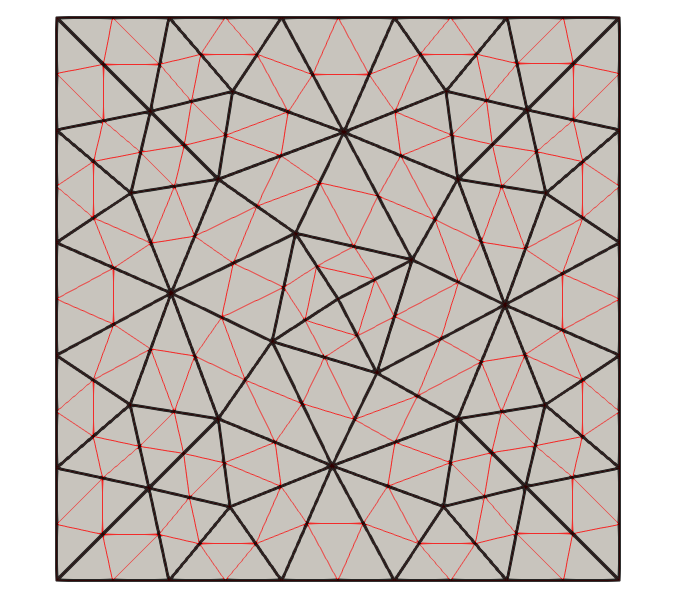
\includegraphics[width=.9\linewidth]{img/refine_unif_mesh.png}
\end{subfigure}%
\begin{subfigure}{.5\textwidth}
\centering
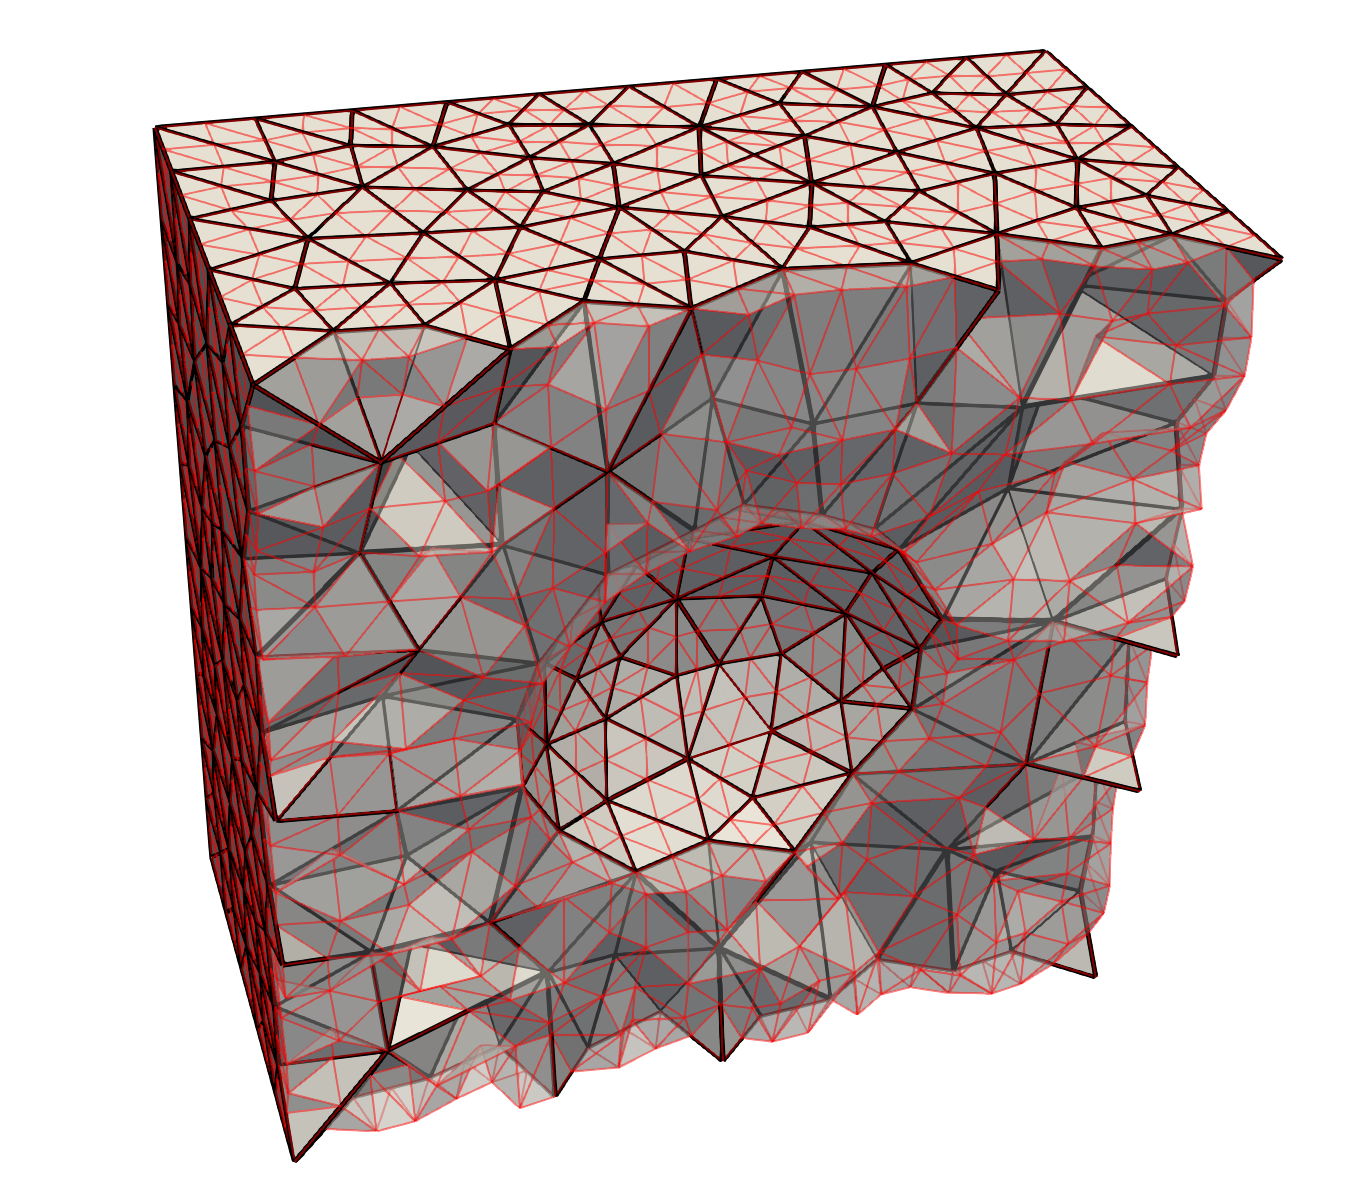
\includegraphics[width=.99\linewidth]{img/refine_unif_mesh_3D.png}
\end{subfigure}
\caption{Edges of a base mesh (black) and a nested mesh refined
with the Unif scheme (red) in two dimensions.}
\label{fig:unif_mesh}
\end{figure}

We first consider the traditional approach of using
a uniformly refined mesh to solve the adjoint problem.
We refer to this approach as the \textsc{Unif}
refinement approach.
To perform uniform refinement, every edge in the mesh
is marked for refinement. The algorithm for uniform
refinement is given in Algorithm \ref{alg:uniform_refine}.
Figure \ref{fig:unif_mesh} demonstrates an example of the
\textsc{Unif} refinement approach applied to a
base mesh. For the uniform refinement approach,
we naturally choose the ration $\frac{h}{H} = \frac12$,
leading to the scaling parameter
$\alpha = 1 - \left( \frac12 \right)^k.$

\begin{algorithm}
\caption{Uniform refinement algorithm}
\begin{algorithmic}
\For{ each edge $e$ in mesh $M$ }
\State mark edge $e$ for refinement.
\EndFor
\end{algorithmic}
\label{alg:uniform_refine}
\end{algorithm}

%%% LONG EDGE REFINEMENT
\subsection{Long Edge Refinement}

\begin{figure}[ht!]
\centering
\begin{subfigure}{.5\textwidth}
\centering
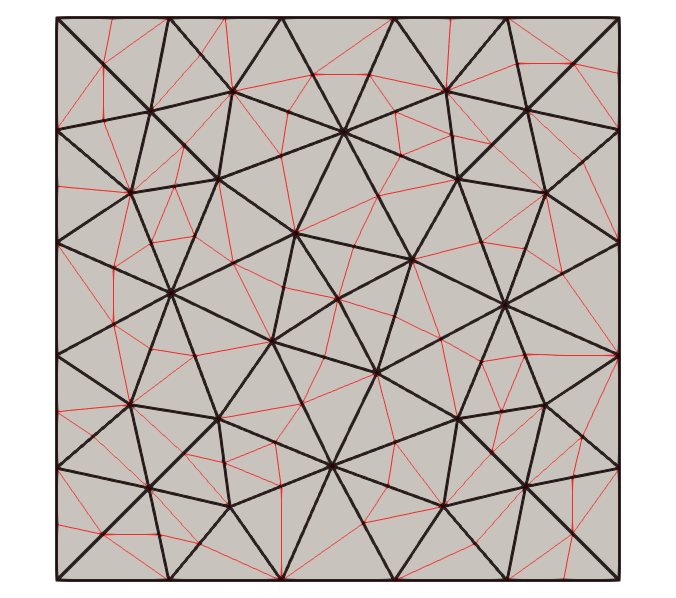
\includegraphics[width=.9\linewidth]{img/refine_long_mesh.png}
\end{subfigure}%
\begin{subfigure}{.5\textwidth}
\centering
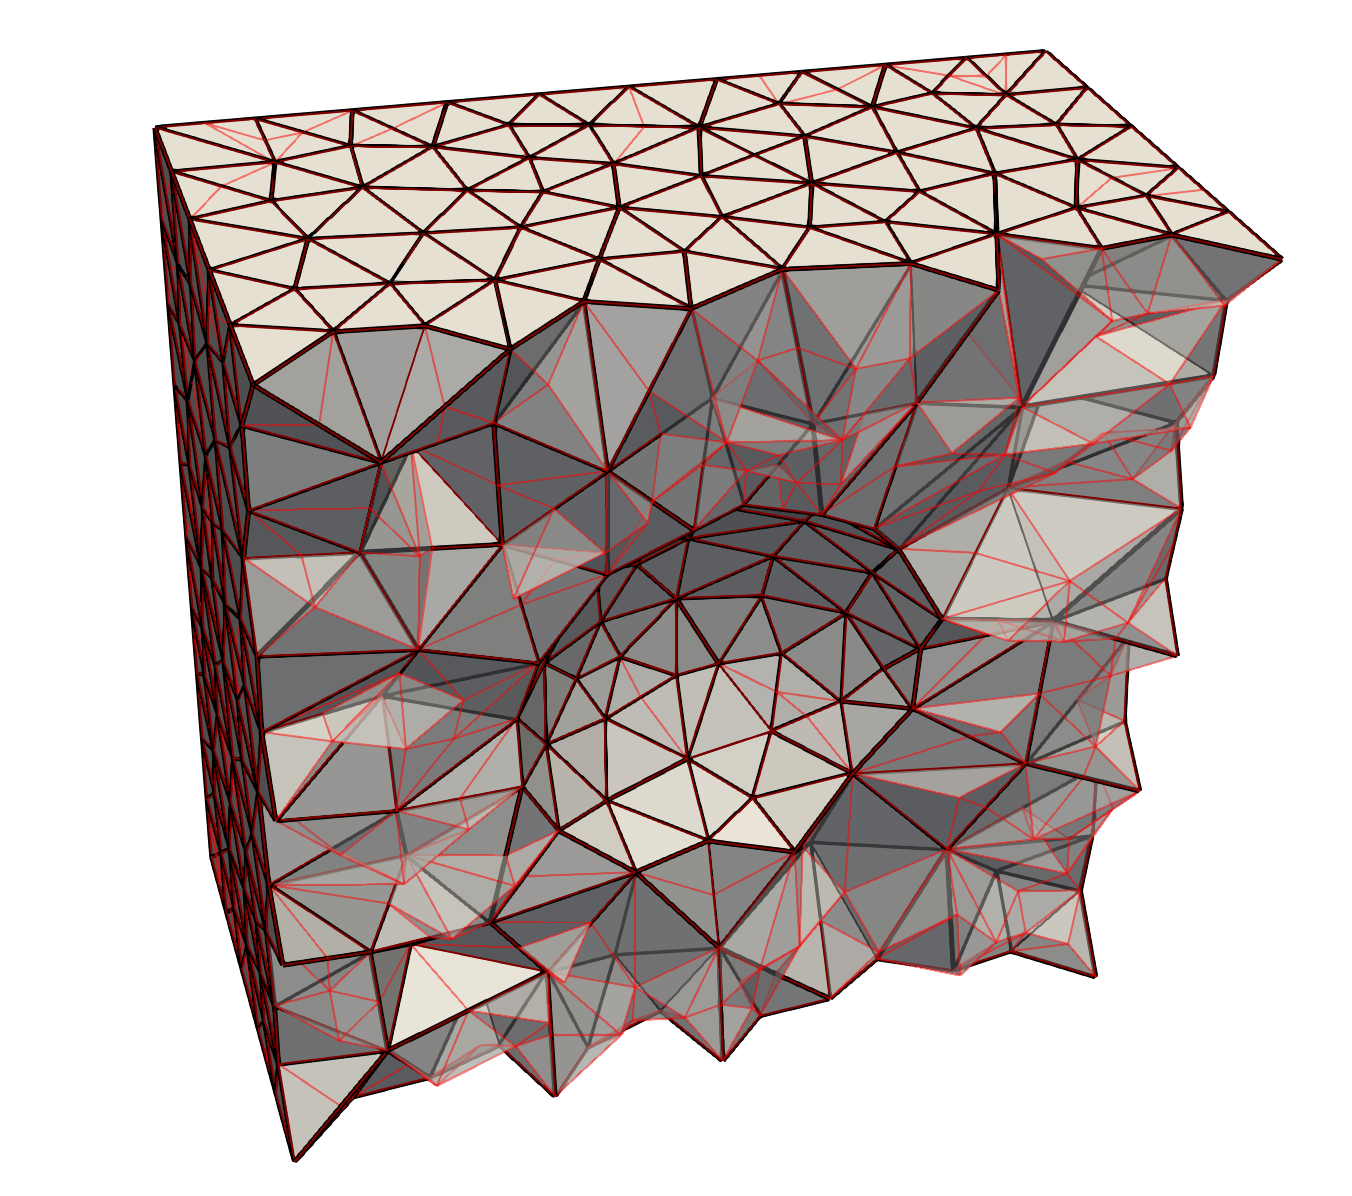
\includegraphics[width=.99\linewidth]{img/refine_long_mesh_3D.png}
\end{subfigure}
\caption{Edges of a base mesh (black) and a nested mesh refined
with the Long scheme (red) in two dimensions.}
\label{fig:long_mesh}
\end{figure}

Next, we consider an adaptive scheme that marks
the longest edge in each element for refinement.
We refer to this scheme as the Long edge
refinement scheme. The \textsc{Long} edge refinement
algorithm is outlined in Algorithm \ref{alg:long_refine}.
Figure \ref{fig:long_mesh} illustrates the
\textsc{Long} edge refinement algorithm applied to
a base mesh.

Note that, for the \textsc{Long} edge refinement
approach, some elements are split once while others
are split multiple times. It follows then that there is
no single global ratio $\frac{h}{H}$ of the fine mesh size
to the coarse mesh size. Presently, we approximate
this ratio by taking the average of all ratios
of nested element sizes to their parent element
size, given by
%
\begin{gather}
\frac{h}{H} \approx \frac{1}{n_{el}}
\sum_{e=1}^{n_{el}} \frac{h_e}{H_e},
\label{eq:refine_ratio}
\end{gather}
%
where $n_{el}$ is the total number of elements
in the nested mesh.

\begin{algorithm}
\caption{Long edge refinement algorithm}
\begin{algorithmic}
\For{ each element $el$ in mesh $M$ }
\For{ each edge $e$ in element $el$ }
\If { $e$ is longest edge in $el$ }
\State mark edge $e$ for refinement.
\EndIf
\EndFor
\EndFor
\end{algorithmic}
\label{alg:long_refine}
\end{algorithm}

%%% SINGLE EDGE REFINEMENT
\subsection{Single Edge Refinement}

\begin{figure}[ht!]
\centering
\begin{subfigure}{.5\textwidth}
\centering
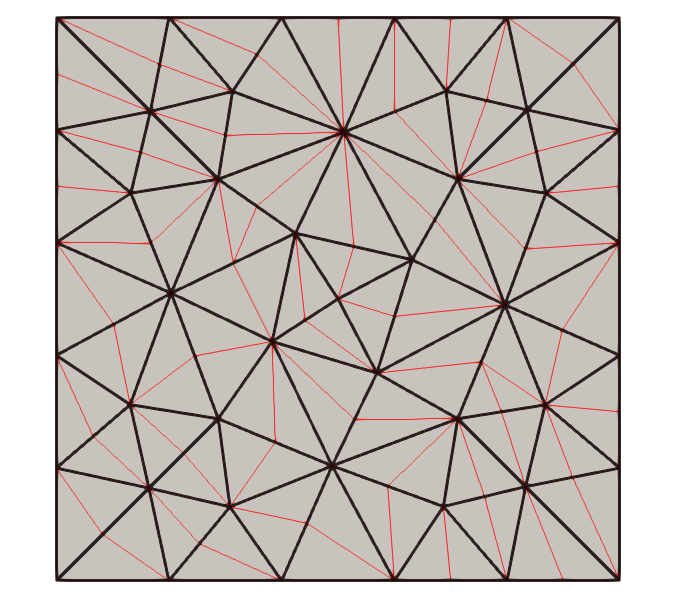
\includegraphics[width=.9\linewidth]{img/refine_single_mesh.png}
\end{subfigure}%
\begin{subfigure}{.5\textwidth}
\centering
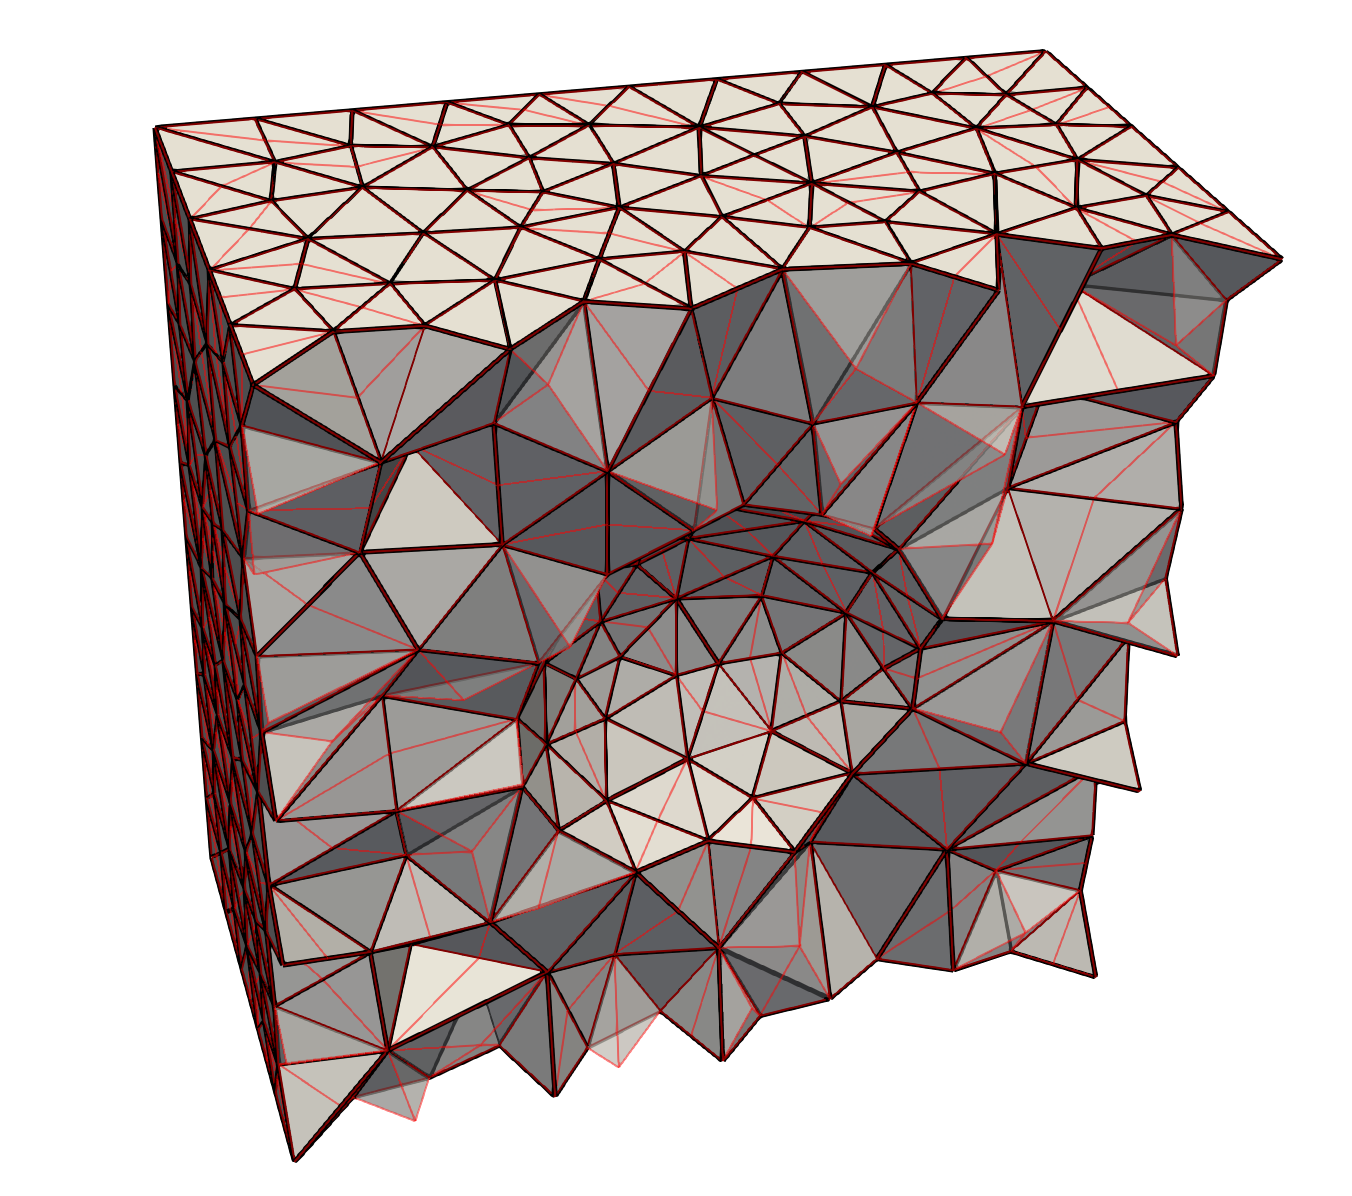
\includegraphics[width=.99\linewidth]{img/refine_single_mesh_3D.png}
\end{subfigure}
\caption{Edges of a base mesh (black) and a nested mesh refined
with the Single scheme (red) in two dimensions.}
\label{fig:single_mesh}
\end{figure}

Finally, we consider a cheap refinement alternative to
uniform refinement that attempts to only mark a single edge
in each element for refinement. We refer to this approach
as the \textsc{Single} edge refinement approach.
To perform single edge refinement, a traversal of all
edges in the mesh is performed. During this traversal,
the first edge encountered is marked for refinement
and the elements adjacent to that edge are tagged
as `visited'. As the edges in the mesh are traversed,
each element adjacent to the edge is checked to see
if it has already been encountered. If all adjacent
elements have not been encountered, then the edge
is marked for refinement.
After this process has completed, some elements may be
\emph{isolated}, in that they have still not been marked as `visited'.
Thus, for each element remaining that has not been marked as `visited',
we mark the first edge adjacent to the element for refinement.
The single edge refinement
algorithm is illustrated in Algorithm \ref{alg:single_refine}.
Figure \ref{fig:single_mesh} demonstrates a mesh
resulting from the application of the single
edge refinement scheme. For the \textsc{Single}
scheme, we again approximate the ratio
$\frac{h}{H}$ with equation \eqref{eq:refine_ratio}.

\begin{algorithm}
\caption{Single edge refinement algorithm}
\begin{algorithmic}
\State initialize all elements to be `not visited'.
\For{ each edge $e$ in mesh $M$ }
\State let $S$ be the set elements adjacent to edge $e$.
\If{ each element in $S$ is `not visited' }
\State mark edge $e$ for refinement.
\For{ each element $el$ in $S$ }
\State mark element $el$ as `visited'.
\EndFor
\EndIf
\EndFor
\For{ each element $el$ in mesh $M$ }
\If{ $el$ is marked as `not visited' }
\State let $S$ be the edges adjacent to element $el$
\State mark the first edge $e$ in $S$ for refinement
\EndIf
\EndFor
\end{algorithmic}
\label{alg:single_refine}
\end{algorithm}

%%% MESH ADAPTATION
\section{Mesh Adaptation}

%%% ERROR LOCALIZATION
\subsection{Error Localization}

It is necessary to localize contributions to the 
total error $\eta$ to mesh entity level \emph{correction indicators}
to drive mesh adaptation. For finite volume and discontinuous
Galerkin finite element methods, it is common to consider the discrete
element-level adjoint weighted residuals of the form
$\bs{z}^h_e \cdot \bs{R}^h_e$, where the subscript $e$ denotes evaluations
over elements. However, for continuous finite elements, this approach
does not account for systematic inter-element cancellation
\cite{fidkowski2011review}, which could lead to a sub-optimal adaptive
strategy.

Traditonally, for continuous Galerkin finite element methods, the
error is localized by integrating the residual by parts to recover
strong form volumetric and jump contributions to the error over
element interiors and boundaries, respectively. Presently, we utilize
a localization strategy introduced by Richter and Wick
\cite{richter2015variational} that proceeds by introducing a
partition of unity $\phi_i$, such that $\sum_i \phi_i = 1$, into the
variational residual. In this localization, adjoint-weighted residual
error information from neighboring elements is gathered to mesh
vertices, leading to vertex-based correction indicators $\eta_i$,
for $i = 1, 2, \dots, n_{vtx}$. Here $n_{vtx}$ denotes the number
of vertices in the fine mesh. To obtain element-level correction
indicators $\eta_e$, where $e = 1,2, \dots, n_{el}$, for the $n_{el}$
elements in the space $\V^H$, we interpolate the vertex-based
indicators $\eta_i$ to element centers in the coarse mesh.
While a full discussion of this localization procedure is outside
of the scope of the present work, we refer readers to
\cite{richter2015variational, wick2016goal} to demonstrate how this
approach is utilized for Galerkin finite element methods and
\cite{granzow2017adjoint} to demonstrate how this approach is
utilized for stabilized finite element methods.

\subsection{Mesh Size Field}

Once element-level correction indicators $\eta_e$ have been obtained, we
drive conforming mesh adaptation by specifying a \emph{mesh size field}.
For isotropic mesh adaptation, which we presently consider, this mesh size
field defines the desired lengths of edges over the mesh. We utilize a mesh
size field as described by Boussetta et al. \cite{boussetta2006adaptive}
that attempts to equidistribute the error in an output adapted mesh with
$N$ target elements. From a high level, this size field will refine the mesh
in areas of the domain that contribute strongly to the error in the functional
and coarsen the mesh in areas of the domain that weakly contribute to the
error in the functional.

Let $p$ be the polynomial interpolant order for the chosen finite element
method. In the subsequent results section, we consider only $p=1$. We first
define the global quantity $G$ as
%
%% refine_global_size
\begin{gather}
G = \sum_{e=1}^{n_{el}} ( \eta_e ) ^{\frac{2d}{2p+d}}.
\label{eq:refine_global_size}
\end{gather}
%
From this global quantity, we compute new element size $H_e^{\text{new}}$
by scaling previous element sizes $H_e$ according to the formula
%
%% refine_size_field
\begin{gather}
H_e^{\text{new}} = \left( \frac{G}{N} \right)^{\frac{1}{d}}
( \eta_e )^{\frac{-2}{2p + d}} H_e.
\label{eq:refine_size_field}
\end{gather}

To ensure that mesh adaptation is being driven by accurate correction indicators
and to prevent excessive coarsening and refinement in a single adaptive step,
we additionally clamp new element sizes such that they are no smaller than one
quarter and no greater than twice the previous element size,
%
%% refine_clamping
\begin{gather}
\frac14 \leq \frac{H_e^{\text{new}}}{H_e} \leq 2.
\label{eq:refine_size_clamping}
\end{gather}

Presently, we make use of the PUMI \cite{ibanez2016pumi} software
for mesh adaptation purposes. This software uses a sequence of edge splits,
swaps, and collapses \cite{li20053d, alauzet2006parallel} to locally modify
the mesh to satisfy the input mesh size field.

%%% RESULTS
\section{Results}

%%% EFFECTIVITY INDICES FOR POISSONS EQUATION
\subsection{Effectivity Indices for Poisson's Equation}

As a first example, we investigate the effectivity of the error estimate
\eqref{eq:refine_error_approx} for the model problem:
%
%% refine_poisson
\begin{gather}
\begin{cases}
\begin{aligned}
- \nabla^2 u &= f \quad &&\bs{x} \in \Omega, \\
u &= 0  \quad &&\bs{x} \in \partial \Omega,
\end{aligned}
\end{cases}
\end{gather}
%
when using the \textsc{Unif}, \textsc{Long}, and \textsc{Single} approaches
to solve the adjoint problem \eqref{eq:refine_adjoint_problem}.
The model problem leads to the Galerkin finite element method: find
$u^H \in \V^H$ such that
%
%% refine_poisson_fem
\begin{gather}
(\nabla w^H, \nabla u^H) = (w, f) \quad \forall w^H \in \V^H,
\label{eq:refine_poisson_fem}
\end{gather}
%
where $(w,u) := \int_{\Omega} w u \, \text{d} \Omega$ denotes the $L^2$ inner
product over the space $\V^H$, defined as
%
%% refine_poisson_space
\begin{gather}
\V^H := \{ u^h \in H^1(\Omega) :
u^H = 0 \; \text{on} \; \partial \Omega \, , \,
u^H |_{\Omega_e} \in \mathbb{P}^1 \}.
\label{eq:refine_poisson_space}
\end{gather}
%
Here $\Omega_e$ denotes an element in a decomposition of the domain
$\Omega$ into $n_{el}$ non-overlapping elements such that
$\cup_{e=1}^{n_{el}} \Omega_e = \Omega$ and
$\Omega_i \cap \Omega_j = \varnothing$ if $i \neq j$.
Additionally,  $\mathbb{P}^1$ denotes the space of piecewise linear
polynomials.

We choose the domain $\Omega = [0,1] \times [0,1]$ and the data
to be $f = 2 \pi^2 \sin(\pi x) \sin(\pi y)$ such that the
exact solution is $u(x,y) = \sin(\pi x) \sin(\pi y)$.
We choose the functional quantity to be
$J(u) = \int_{\Omega} u \, \text{d} \Omega$, which has the exact
value $J(u) = \frac{4}{\pi^2}$.
With the proposed finite element method, we
expect the functional to converge at the rate
$k=2$, which we use to determine the scaling parameter
$\alpha$ as given by equation \eqref{eq:refine_alpha}.

The model problem was solved with mesh sizes
$H = \{\frac{1}{5}, \frac{1}{10}, \frac{1}{20},
\frac{1}{40}, \frac{1}{80}, \frac{1}{160} \}$.
For each chosen mesh size, the discrete
adjoint problem \eqref{eq:refine_adjoint_problem}
was solved on fine spaces $\V^h$
generated by the \textsc{Unif},
\textsc{Long}, and \textsc{Single} refinement
schemes. An error estimate for the three schemes
is then computed according to equation
\eqref{eq:refine_error_approx}.

\begin{figure}[ht!]
\centering
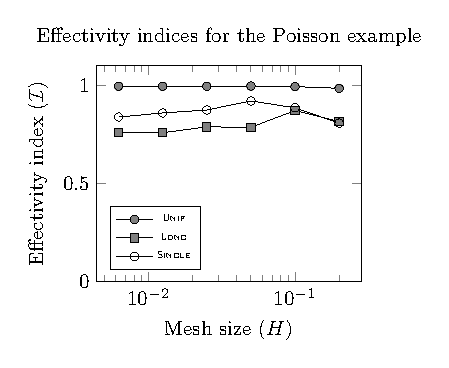
\includegraphics[width=0.5\textwidth]{img/refine_poisson_effectivity}
\caption{Effectivity indices using the Unif,
Long, and Single refinement schemes for
the Poisson example problem}
\label{fig:refine_poisson_effectivity}
\end{figure}

Figure \ref{fig:refine_poisson_effectivity} plots
the effectivity index \eqref{eq:refine_effectivity}
for each of the three schemes at each chosen
mesh size. Effectivity indices for the
baseline \textsc{Unif} method approach
$1$ in the limit as $H \to 0$ as expected. The effectivity
indices obtained using the two non-uniform refinement approaches,
are less accurate
and do not appear to be asymptotically correct.
This is perhaps not surprising, as we have considered a bulk
average for the ratio $\frac{h}{H}$ for these two schemes,
as shown in Table \ref{tab:refine_poisson_ratios}.

%
%% refine_poisson_ratios
\begin{table}[ht!]
\centering
\begin{tabular}{ | c | c | c | } \hline
$H$ & \textsc{Long} : $\frac{h}{H}$ & \textsc{Single} : $\frac{h}{H}$ \\ \hline \hline
$\frac{1}{5}$ & 0.6344 & 0.8198 \\ \hline
$\frac{1}{10}$ & 0.6323 & 0.8212 \\ \hline
$\frac{1}{20}$ & 0.6325 & 0.8204 \\ \hline
$\frac{1}{40}$ & 0.6490 & 0.8183 \\ \hline
$\frac{1}{80}$ & 0.6477 & 0.8202 \\ \hline
$\frac{1}{160}$ & 0.6467 & 0.8195 \\ \hline
\end{tabular}
\caption{Approximated mesh size ratios for the Long and
Single schemes for the first Poisson's equation example.}
\label{tab:refine_poisson_ratios}
\end{table}

However, even though the error estimates themselves obtained by
the \textsc{Long} and \textsc{Single} schemes may not be suitable
for application purposes, these schemes may still be suitable to
drive mesh adaptation at a cheaper cost than the full \textsc{Unif}
approach. Figure \ref{fig:refine_poisson_dofs}
demonstrates the decrease in the total number of degrees of
freedom for the adjoint problem for the \textsc{Long} and \textsc{Single}
schemes as compared to the \textsc{Unif} scheme. This motivates
us to consider an adaptive example for Poisson's equation in the
next section.

%
%% refine_poisson_dofs
\begin{figure}[ht!]
\centering
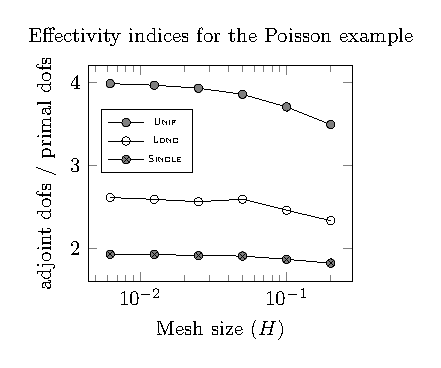
\includegraphics[width=0.5\textwidth]{img/refine_poisson_dofs}
\caption{Ratio of adjoint problem degrees of freedom to primal
problem degrees of freedom using the Unif,
Long, and Single refinement schemes
for the Poisson example problem}
\label{fig:refine_poisson_dofs}
\end{figure}

%%% Mesh Adaptation for Poisson's Equation
\subsection{Mesh Adaptation for Poisson's Equation}

In this example, we again consider the governing equations for Poisson's
equation, as given in the previous section. However, we now choose the
forcing function $f$ to be $f=1$ and the domain
$\Omega := [-1,1] \times [-1,1] \setminus
[-\frac12, \frac12] \times [-\frac12, \frac12]$. Further, we consider
the point-wise quantity of interest
$J(u) = \int_{\Omega} \delta(\bs{x} - \bs{x}_0) u \, \text{d} \Omega$,
where the point of interest is chosen to be
$\bs{x}_0 = (0.75, 0.75)$. We again expect the functional to converge
at the rate $k = 2$. The domain and point-wise QoI location are show
in Figure \ref{fig:refine_poisson2_geom}. The value of the quantity
of interest was determined to have a value of $J(u) = 0.0334473
\pm 1e\mbox{-}7$ in the reference \cite{dealiistep14}.

%
%% refine_poisson2_geom
\begin{figure}[ht!]
\centering
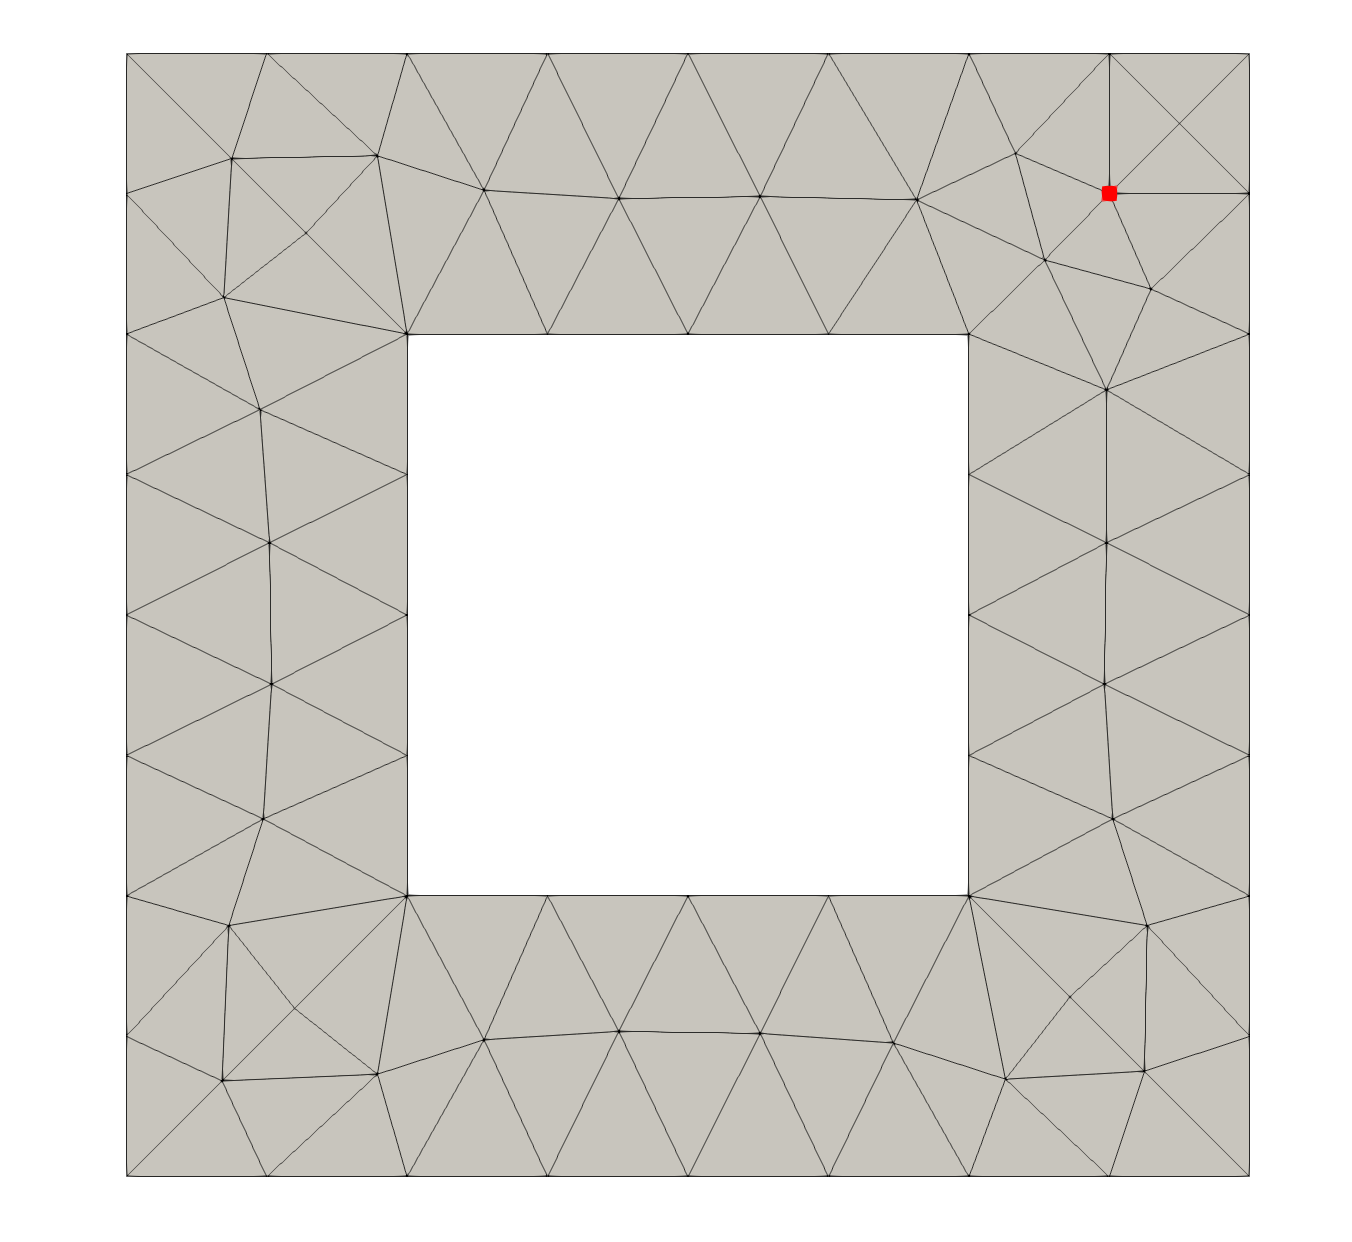
\includegraphics[width=0.4\textwidth]{img/refine_squarehole_initial.png}
\caption{Geometry and initial mesh used for the second Poisson's
equation example with the point of interest shown in red.}
\label{fig:refine_poisson2_geom}
\end{figure}

We performed the steps:
\begin{gather*}
\text{Solve Primal} \rightarrow \text{Solve Adjoint} \rightarrow
\text{Estimate Error} \rightarrow \text{Adapt Mesh}
\end{gather*}
7 times, starting from the initial mesh shown in Figure
\ref{fig:refine_poisson2_geom}. We solve the adjoint problem with
three different methods on nested meshes obtained with the
\textsc{Unif}, \textsc{Long}, and \textsc{Single} refinement
schemes. At each adaptive step, the mesh size field was set
according to equation \eqref{eq:refine_size_field}, such that
the target number of elements $N$ is twice that of the current
mesh.

%
%% squarehole_convergence
\begin{figure}[ht!]
\centering
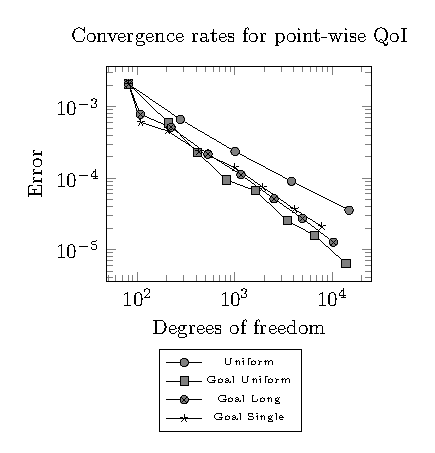
\includegraphics[width=.5\linewidth]{img/refine_squarehole_convergence.pdf}
\caption{Error evolution for adaptive schemes for the second Poisson's equation
example.}
\label{fig:squarehole_convergence}
\end{figure}

Figure \ref{fig:squarehole_convergence} illustrates the convergence
history for the error $J(u) - J(u^H)$ for the three adaptive schemes
obtained with the \textsc{Unif} (Goal Uniform), the \textsc{Long}
(Goal Long), and the \textsc{Single} strategies,
along with the error obtained by solving the primal problem with
successively uniformly refined meshes (Uniform). The rate of
convergence for the \textsc{Unif} scheme agrees with the
reference \cite{dealiistep14}. Additionally, the error for
both the \textsc{Long} and \textsc{Single} schemes converges at a
rate almost near the \textsc{Unif} scheme.

%
%% refine_unif_adapted
\begin{figure}[ht!]
\centering
\begin{subfigure}{.5\textwidth}
\centering
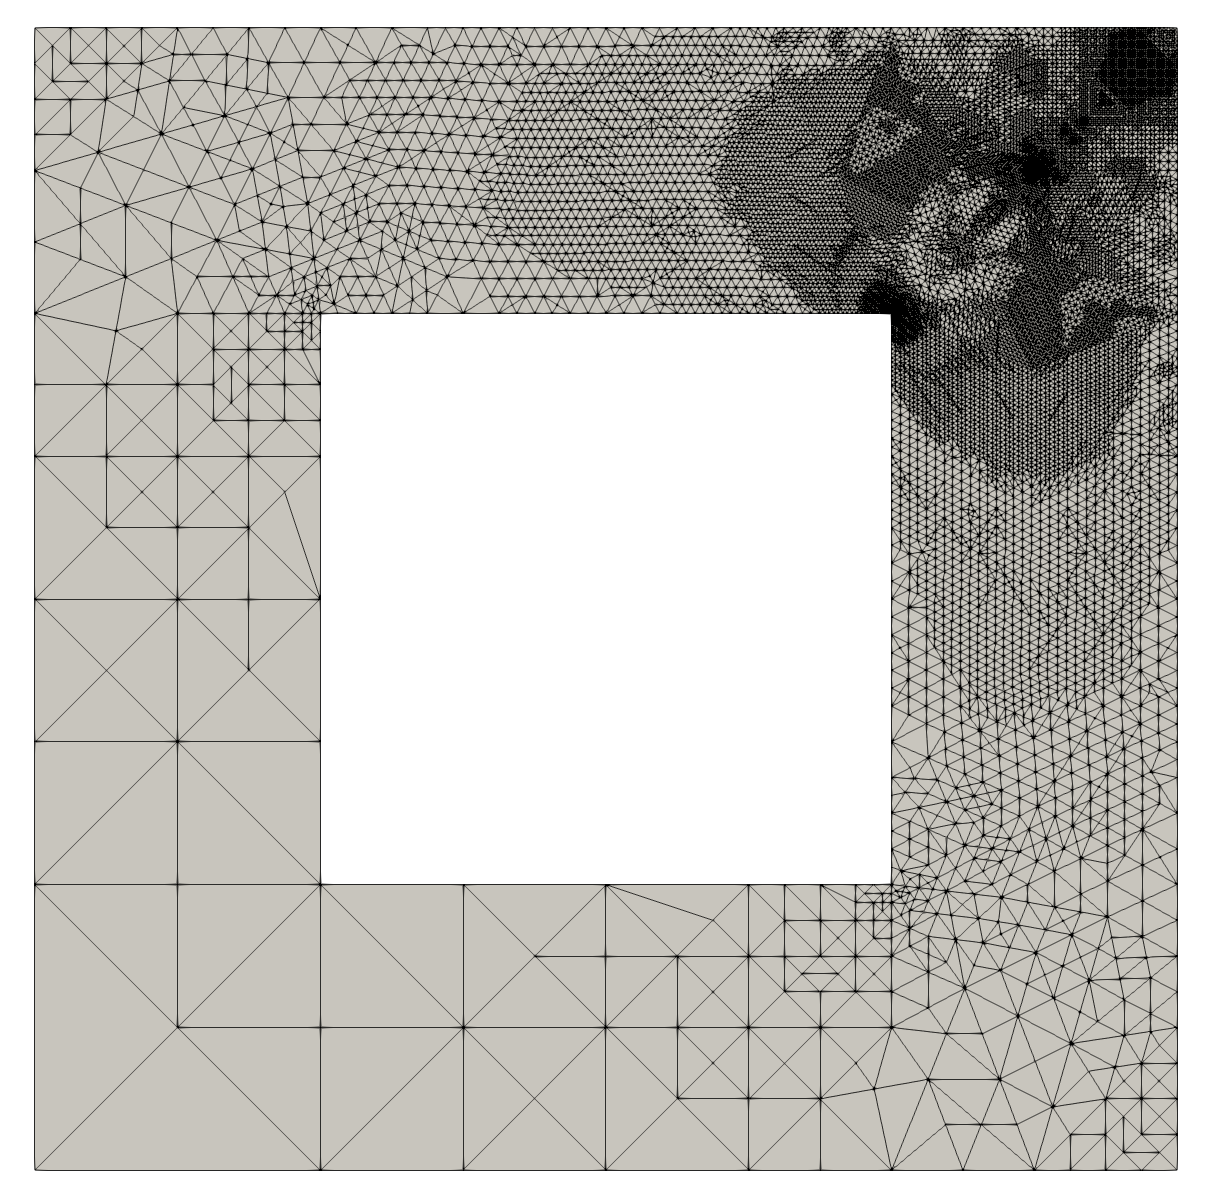
\includegraphics[width=.99\linewidth]{img/refine_squarehole_unif.png}
\end{subfigure}%
\begin{subfigure}{0.5\textwidth}
\centering
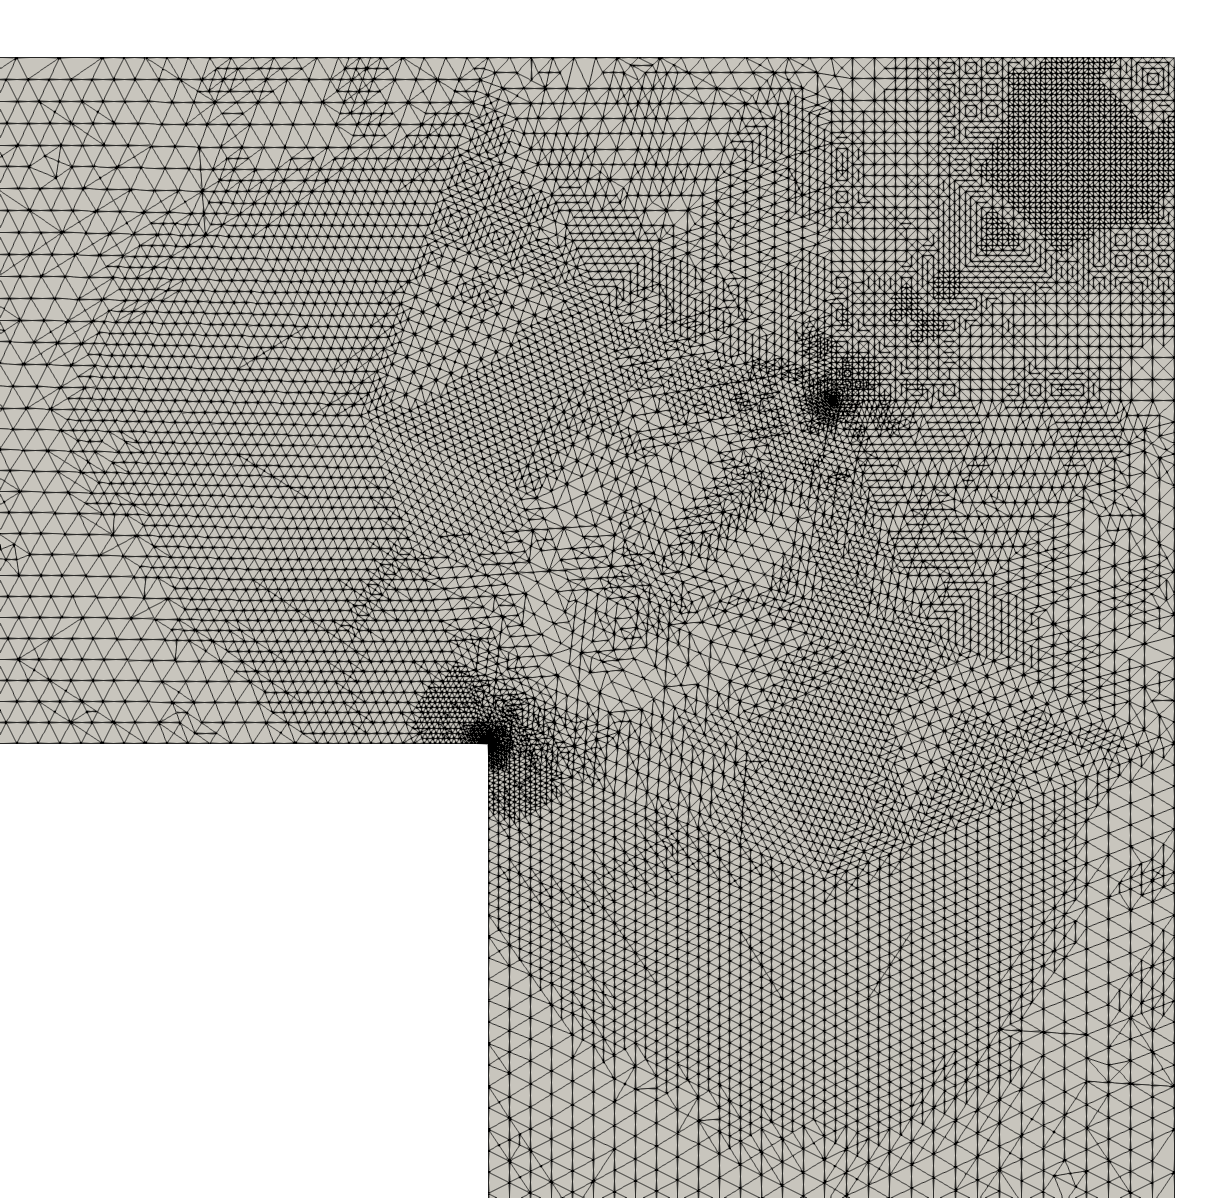
\includegraphics[width=.99\linewidth]{img/refine_squarehole_unif_close.png}
\end{subfigure}
\caption{The final adapted mesh using the Unif strategy to
solve the adjoint problem (left) and a close-up of the upper right-hand
corner of this mesh (right).}
\label{fig:refine_unif_adapted}
\end{figure}

Figure \ref{fig:refine_unif_adapted} illustrates the final adapted mesh
obtained using the \textsc{Unif} strategy to solve the adjoint problem.
The distribution of degrees of freedom in this mesh closely resemembles
the results obtained in reference \cite{dealiistep14}. However, using
the \textsc{Long} and \textsc{Single} to solve the adjoint problem
results in final adapted meshes that appear to be largely
unsuitable for application analysis, as shown in Figures
\ref{fig:refine_long_adapted} and
\ref{fig:refine_single_adapted}, even thought these meshes result
in more accurate functional evaluations as compared to uniform
refinement.

%
%% refine_long_adapted
\begin{figure}[ht!]
\centering
\begin{subfigure}{.5\textwidth}
\centering
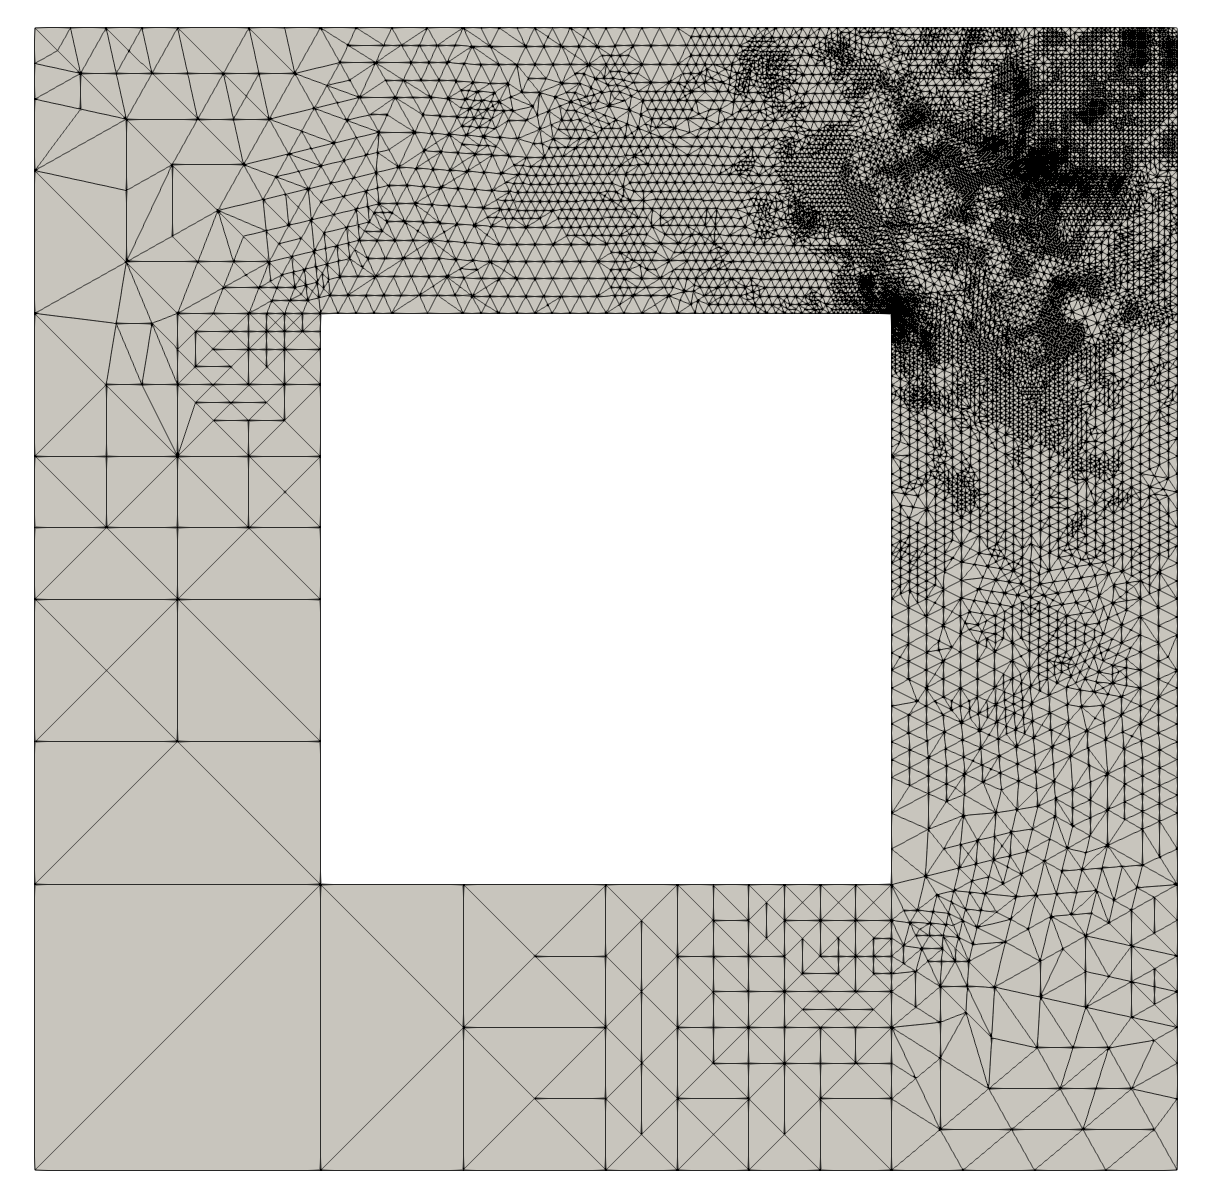
\includegraphics[width=.99\linewidth]{img/refine_squarehole_long.png}
\end{subfigure}%
\begin{subfigure}{0.5\textwidth}
\centering
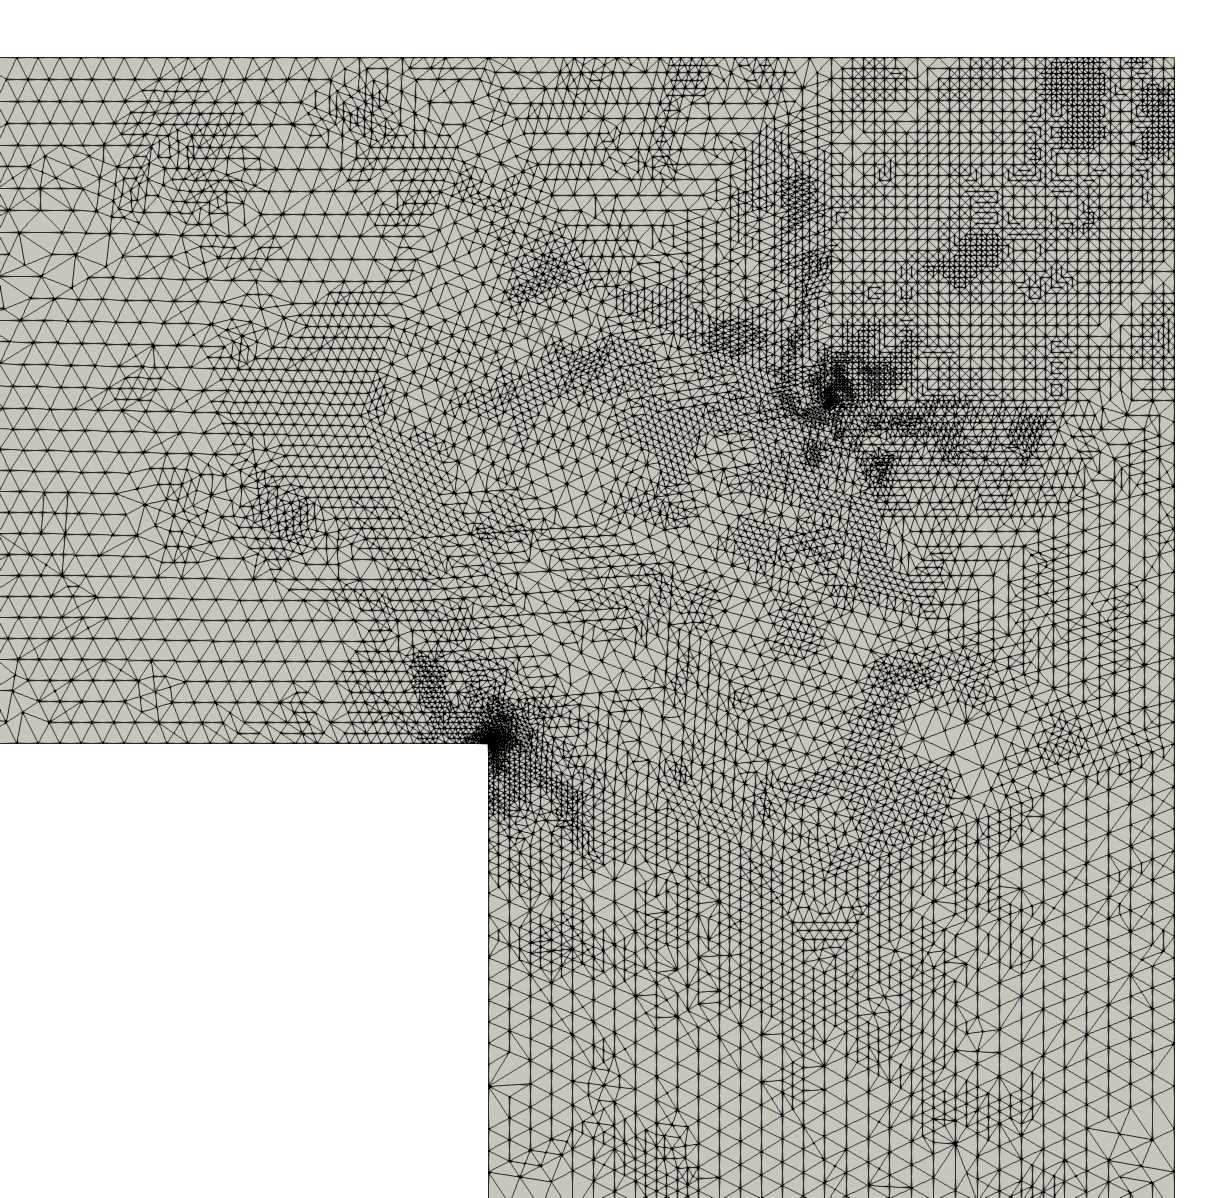
\includegraphics[width=.99\linewidth]{img/refine_squarehole_long_close.png}
\end{subfigure}
\caption{The final adapted mesh using the Long strategy to
solve the adjoint problem (left) and a close-up of the upper right-hand
corner of this mesh (right).}
\label{fig:refine_long_adapted}
\end{figure}

%
%% refine_single_adapted
\begin{figure}[ht!]
\centering
\begin{subfigure}{.5\textwidth}
\centering
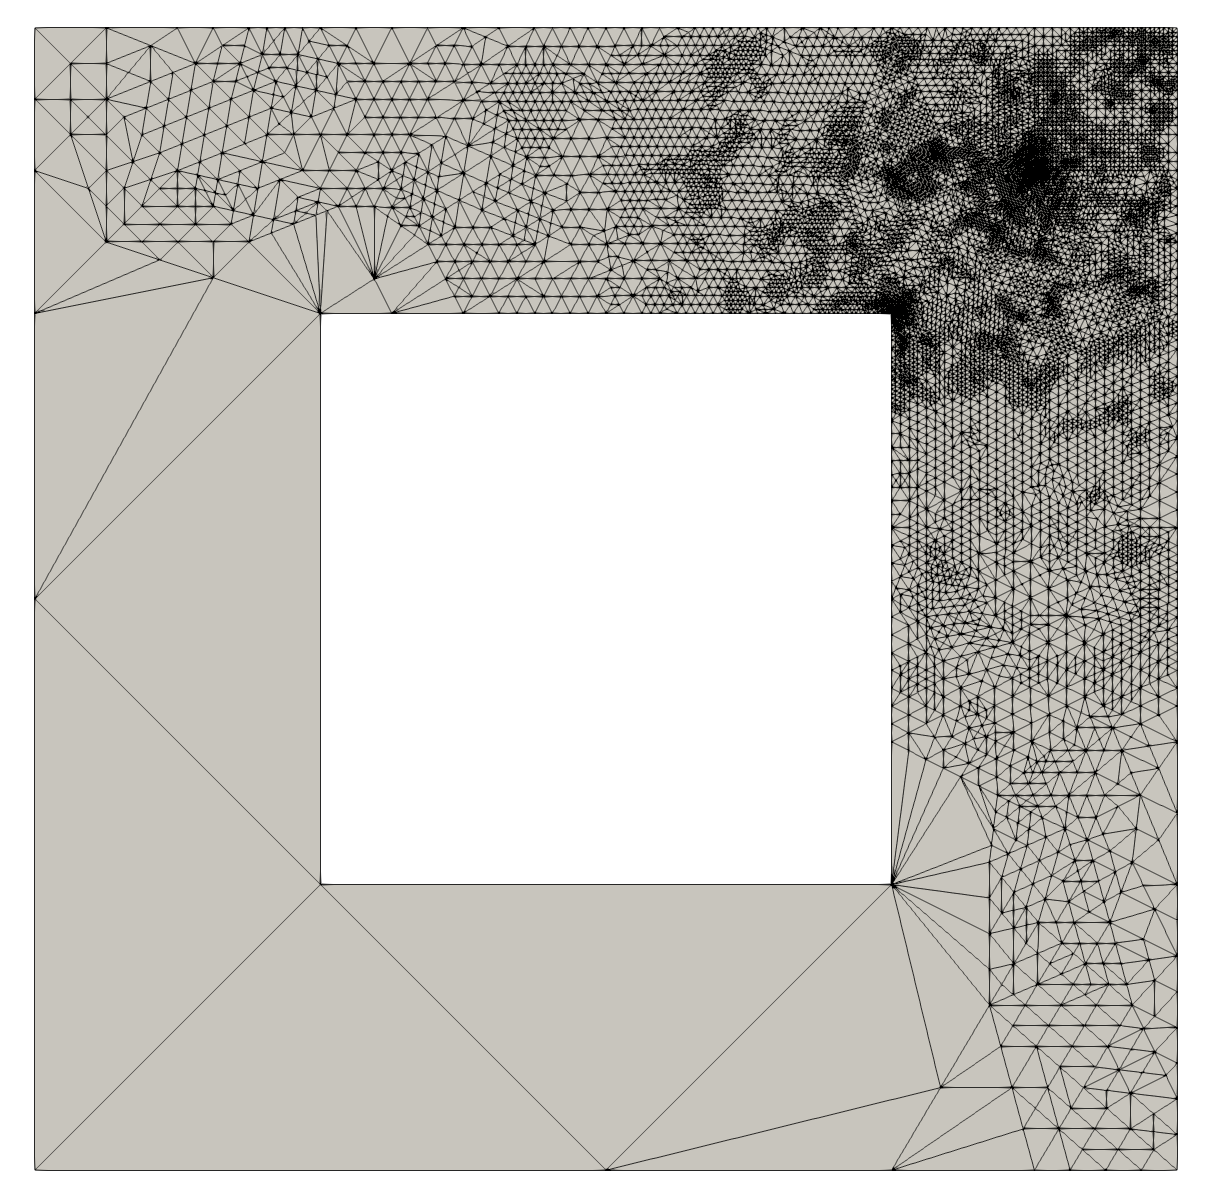
\includegraphics[width=.99\linewidth]{img/refine_squarehole_single.png}
\end{subfigure}%
\begin{subfigure}{0.5\textwidth}
\centering
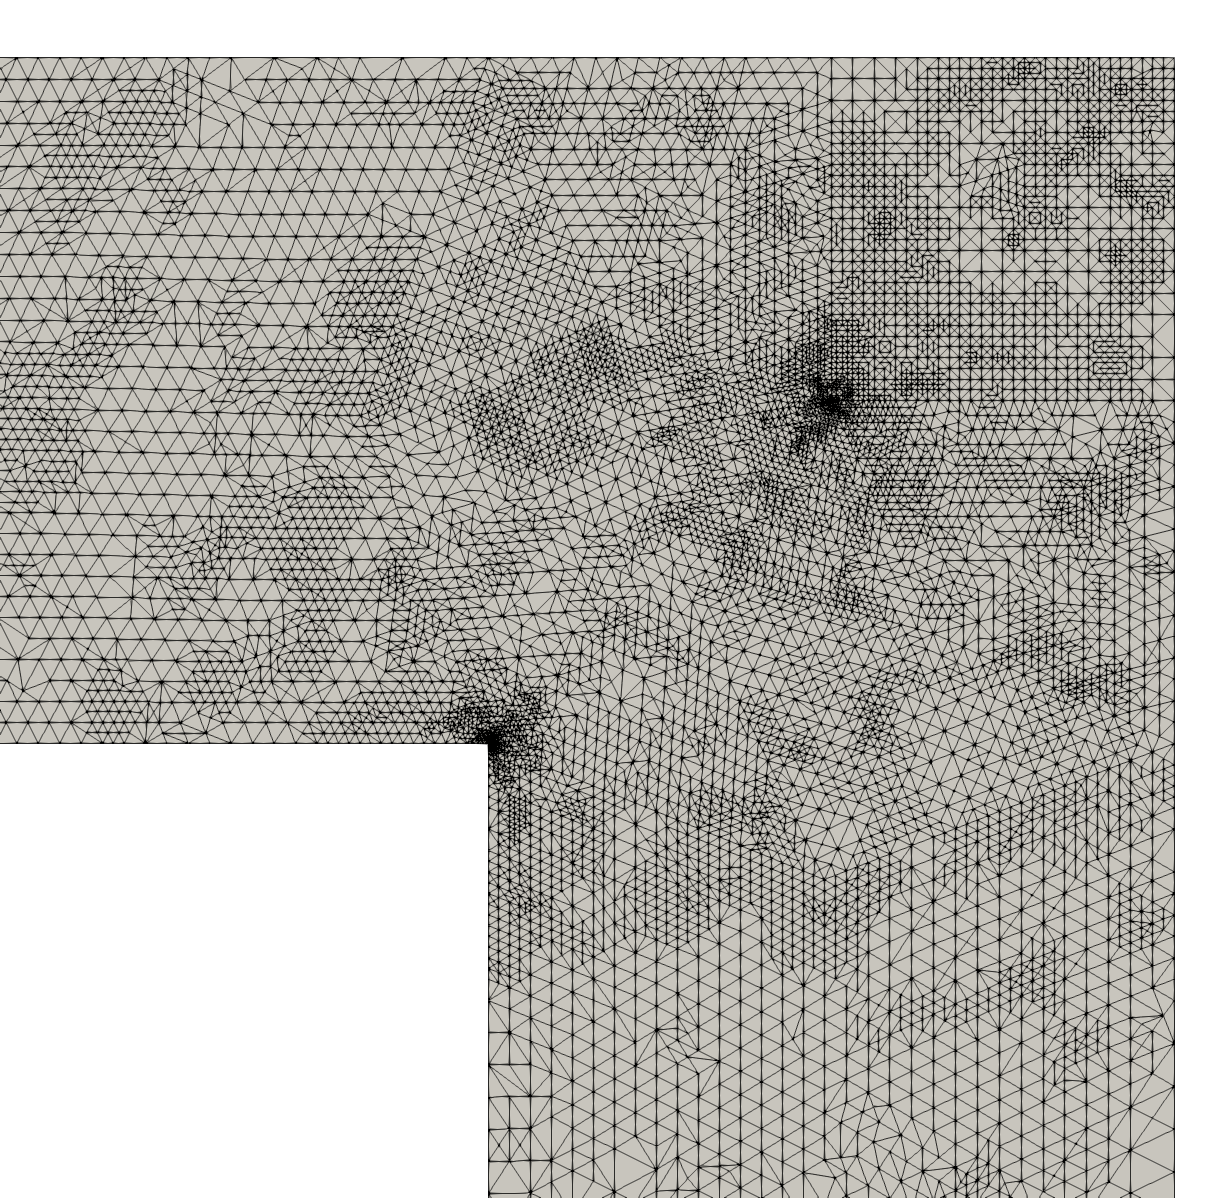
\includegraphics[width=.99\linewidth]{img/refine_squarehole_single_close.png}
\end{subfigure}
\caption{The final adapted mesh using the Single strategy to
solve the adjoint problem (left) and a close-up of the upper right-hand
corner of this mesh (right).}
\label{fig:refine_single_adapted}
\end{figure}

%%% CONCLUSIONS
\section{Conclusions and Outlook}

We have developed two alternative approaches to uniform refinement
for performing enriched adjoint solves in adjoint-based error estimation
with two discretization levels. We have applied this approach to
Poisson's equation. While the number of
degrees of freedom for the adjoint solve for these two
alternative approaches decreases significantly when compared to the
more traditional approach of solving the adjoint problem on
a uniformly refined mesh, the present outlook indicates that
these approaches are not yet suitable for practical applications.
That is, when performing adjoint-based error estimation with the
two novel approaches, effectivity indices are not asymptotically
correct. Additionally, the meshes obtained with adaptive adjoint-based
analysis display qualitatively different features when
compared to the uniform refinement approach.

It is possible that more accurate error estimates could be
obtained by considering the total functional error as the sum
of element-level contributions
\begin{gather}
J^h(u^h) - J^h(u^h_H) \approx \sum_{e=1}^{n_{el}}
- \frac{1}{\alpha_e} \bs{z}^h_e \cdot \bs{R}^h_e(\bs{u}^h_H),
\end{gather}
where we have replaced the approximated ratio
\eqref{eq:refine_ratio} with the exact element-level
ratio, $\alpha_e = 1 - \left( \frac{h_e}{H_e} \right)^k$. Here, the
subscript $e$ denotes the element-level contributions
to the corresponding global quantity. Additionally, it is
possible that more suitable meshes may be obtained during
the adaptive process if a size field smoothing
algorithm is utilized. We leave investigation into these
areas as a suggestion for future work.
